\chapter{Spectral data}
\label{ch:spectral-data}

\begin{marginfigure}
%   \centering
  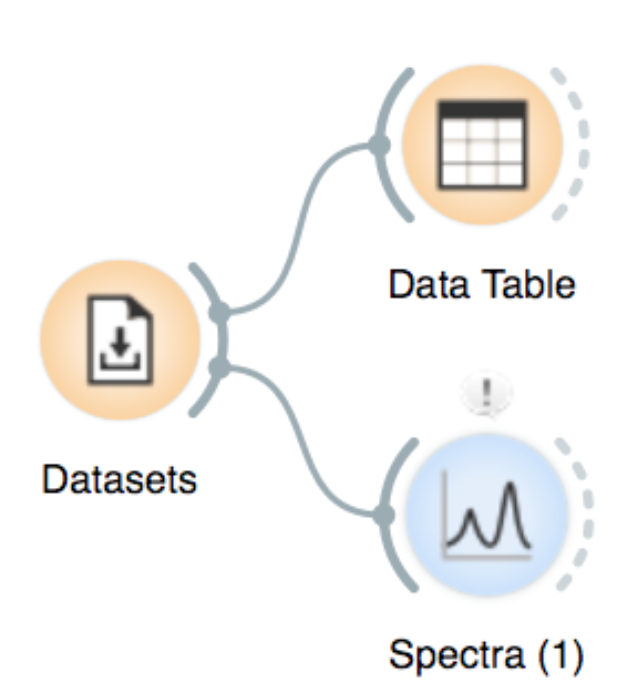
\includegraphics[width=40mm]{spectral-data-fig1.png}%
  \caption{Your first spectroscopy workflow!}
  \label{fig:spectral-data-fig1}
\end{marginfigure}

\newthought{Let's make the small workflow} shown on the right and open the “Liver spectroscopy” data set from \mutation’s \textit{Datasets} widget.
In a \textit{Data Table}, each row represents a spectrum. For the liver dataset, all columns, except the class column, describe absorbance at a specific wavenumber. Their column names must be numbers, otherwise \mutation’s spectral tools will just enumerate them, starting from 0.

\begin{figure}[h]
  \centering
  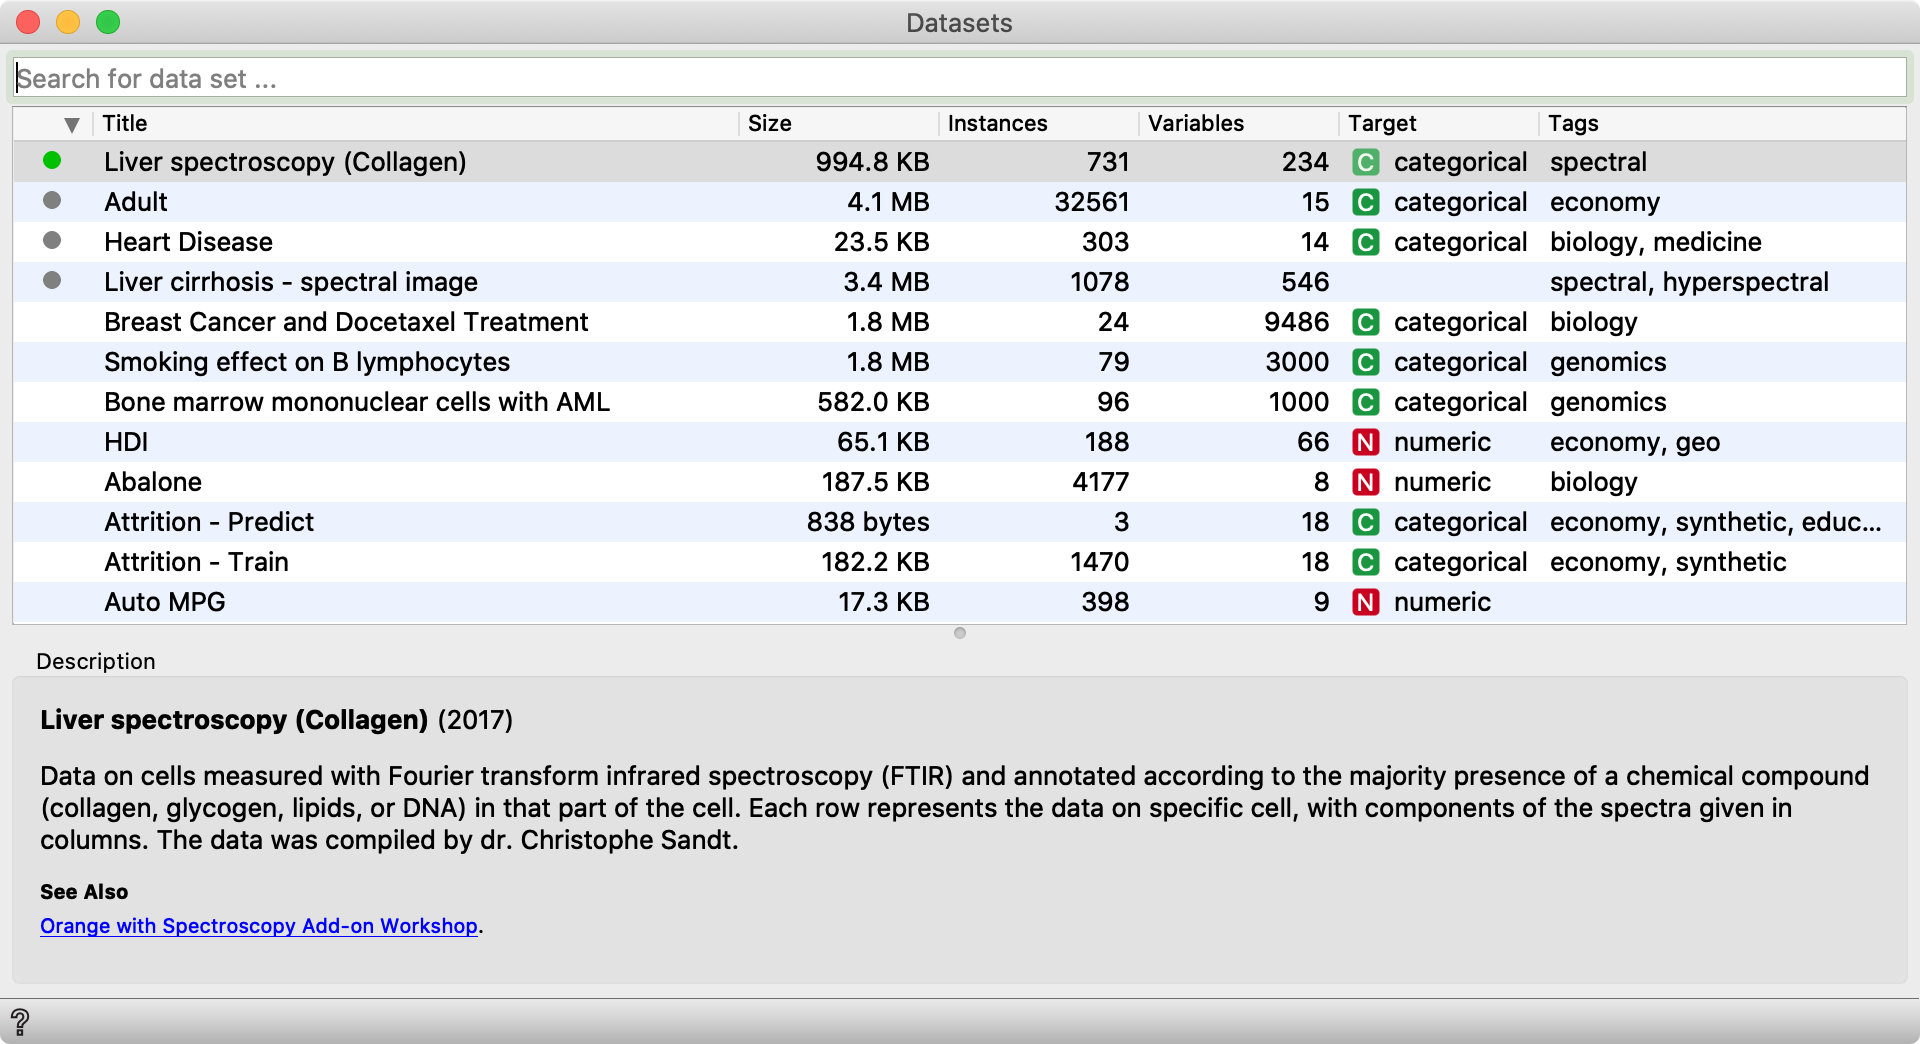
\includegraphics[width=\linewidth]{spectral-data-fig2.png}%
  \caption{The \textit{Datasets} widget provides data for training and testing purposes. The files are stored on a server and to use it, you need a working internet connection, but after you accessed them, they are stored on your computer for off-line use.}
  \label{fig:spectral-data-fig2}
\end{figure}

Connect the data to a \textit{Spectra} widget from the \textbf{Spectroscopy} toolbox. To see the graph below, choose the feature for coloring in the top-left Menu (or click on the graph and press “c”).

\begin{marginfigure}
  \centering
  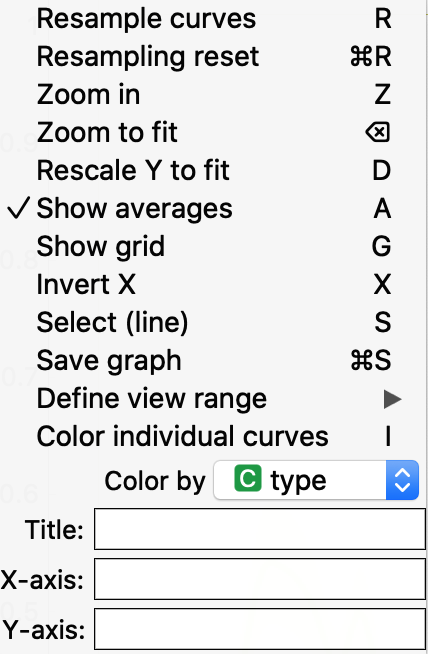
\includegraphics[width=35mm]{spectral-data-fig4.png}
  \caption{The \textit{Spectra} widget and it's options. Try to use keyboard shortcuts on the right for frequent actions.}
  \label{fig:spectral-data-fig4}
\end{marginfigure}

\begin{figure}[h]
  \centering
  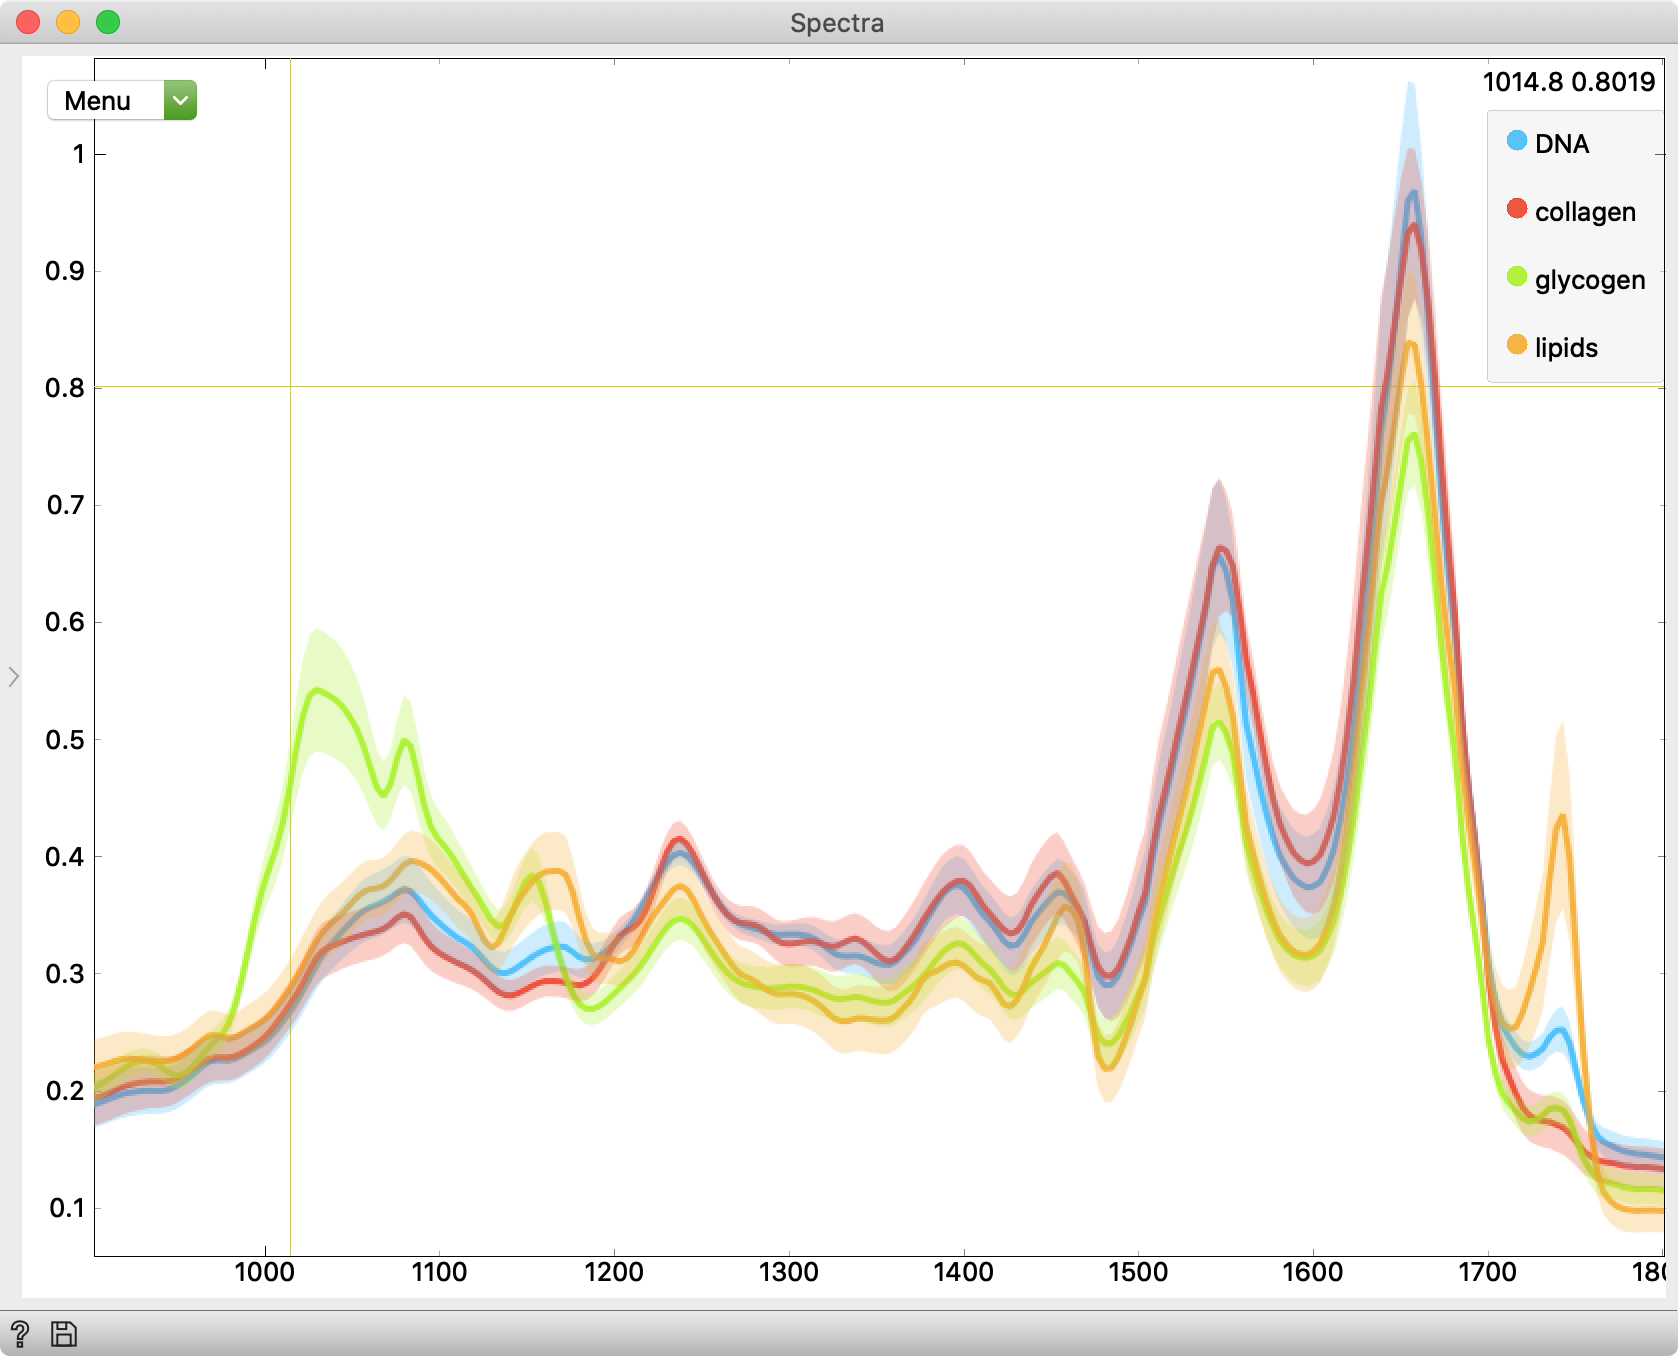
\includegraphics[width=70mm]{spectral-data-fig3.png}%
  \caption{$\;$}  % empty caption for correct figure placement
  \label{fig:spectral-data-fig3}
\end{figure}
